% !TEX root = ../main.tex
\section{Symmetry-reduced domain}\label{sec:symmetry-reduced-domain}

The RID's symmetries introduce redundancy into the configuration space.
We can use this redundancy to restrict the parameter ranges for the viewing
direction and relative rotation to a small bounded region, while retaining
at least one representative of every configuration. This reduction also
justifies using the parametrisation of
\cref{subsec:parametrisation-of-the-configuration-space}: viewing directions
and relative rotations that it does not represent directly have equivalent
representatives within the chosen parameter ranges.

\subsection{Symmetries preserve the projection problem}\label{subsec:symmetries-preserve-the-projection-problem}

A \emph{body symmetry} is an orthogonal linear map taking $\mathcal R$ to itself.
Orientation-preserving body symmetries have determinant $1$ and are rotations;
orientation-reversing symmetries have determinant $-1$.
An orientation-reversing symmetry that fixes a plane pointwise is a
\emph{reflection}. Let $\mathcal G$ be the group of rotation symmetries.
Applying one of these to the plug before its
relative rotation does not change the plug at all: for $G_{P}\in\mathcal G$,
$R_{P}G_{P}\mathcal R=R_{P}\mathcal R$. Applying a hole symmetry $G_{H}\in\mathcal G$ to the whole
configuration also leaves the hole fixed as $\mathcal R$, while rotating the
viewing direction and plug together.

These two operations replace the viewing vector and relative rotation by
\[
  (\mathbf u,R_{P})\longmapsto(G_{H}\mathbf u,G_{H}R_{P}G_{P}),
  \qquad G_{H},G_{P}\in\mathcal G.
\]
Orthogonal projection respects this common change of frame:
\[
  \pi_{G_{H}\mathbf u}(G_{H}\mathbf v)=G_{H}\pi_{\mathbf u}(\mathbf v).
\]
Consequently, the two new shadows are the images of the old shadows under
the same planar isometry. Every containment comparison, including after
scaling either shadow by $\lambda>0$, is preserved. By
\cref{lem:margin-and-containment}, the margin is unchanged, as are the
truth values of the fit, touch and poke predicates.

We can also use the orientation-reversing symmetries. Since $\mathcal R=-\mathcal R$, any such
symmetry $G_{H}$ has $-G_{H}\in\mathcal G$.
Applying $-G_{H}$ instead keeps the plug's transformation a rotation, and its viewing
vector $-G_{H}\mathbf u$ represents the same line as $G_{H}\mathbf u$.
Thus all orthogonal body symmetries are available when choosing the
viewing line. They form $\mathcal G\cup(-\mathcal G)$.

Choosing the sign of the viewing vector also lets us make its $z$-coordinate
positive whenever it is nonzero, as assumed in the parametrisation of
\cref{subsec:parametrisation-of-the-configuration-space}. Viewing lines in
the $xy$-plane will be handled by the reduction in
\cref{subsec:rotation-and-reflection-reduction}.

\paragraph{The finite symmetry group.}
The RID has icosahedral symmetry, so $\mathcal G$ contains 60 rotations
and $-\mathcal G$ contains 60 orientation-reversing symmetries, including
15 planar reflections. Let $\mathcal Q$ be the set of unit quaternions representing
the rotations in $\mathcal G$, with both signs $g$ and $-g$ included for
each rotation. Thus $\mathcal Q$ has 120
members, whose coordinates belong to $\mathbb Q(\sqrt5)$. It includes all
eight signed coordinate-unit quaternions: one coordinate is $1$ or $-1$
and the other three are zero. The two signs represent the same rotation;
composing that rotation with central inversion gives its
orientation-reversing counterpart.
The quaternion families and exact checks establishing these finite facts
and the full symmetry count are given in
\cref{app:quaternion-families-and-the-full-symmetry-group}.

\subsection{Rotation and reflection reduction}\label{subsec:rotation-and-reflection-reduction}

We first restrict the viewing line, then keep its representative vector
$\mathbf u$ fixed while choosing the relative rotation. The reflection planes divide the viewing directions
into equivalent regions. We will select a representative in one closed
triangular region, including its boundary.

Reflections arise from the members of $\mathcal Q$ whose scalar part is zero. A unit quaternion
$(0,\mathbf n)$ represents the half-turn $2\mathbf n\mathbf n^{\mathsf T}-I$.
Its negative as a spatial matrix is the reflection
\[
  S_{\mathbf n}=I-2\mathbf n\mathbf n^{\mathsf T},
\]
which is a body symmetry by central inversion. There are 15 such normal
lines. Choose $\mathbf h=(1,2,9)$ and orient each unit normal so that
$\mathbf h\cdot\mathbf n>0$; none is perpendicular to $\mathbf h$.
This auxiliary vector chooses which side of each reflection plane we retain.

Among the images of a nonzero viewing vector under all 120 orthogonal symmetries,
choose one, still denoted by $\mathbf u$, that maximises
$\mathbf h\cdot\mathbf u$. If $\mathbf n\cdot\mathbf u<0$ for any of the
oriented normals, its reflection would give
\[
  \mathbf h\cdot(S_{\mathbf n}\mathbf u-\mathbf u)
    =-2(\mathbf h\cdot\mathbf n)(\mathbf n\cdot\mathbf u)>0,
\]
contradicting maximality. Thus the chosen vector $\mathbf u$ lies on the retained side
of every reflection plane.

\paragraph{The viewing triangle.}
Writing $\mathbf u=(u_1,u_2,u_3)$, the intersection of these 15 closed
halfspaces is exactly the cone
\begin{equation}\label{eq:viewing-cone}
  u_1\ge0,\qquad u_2\ge0,\qquad
  u_3\ge\varphi u_1+\varphi^2u_2.
\end{equation}
The equivalence between these halfspace conditions and the three cone
inequalities is proved in \cref{app:reflection-normals-and-the-viewing-cone}.

A nonzero vector in the cone has positive $z$-coordinate, so we can divide
by $u_3$ and write $\mathbf u=(s,t,1)$. The retained parameter pairs $(s,t)$
form the closed triangle
\begin{equation}\label{eq:viewing-triangle}
  s\ge0,\qquad t\ge0,\qquad \varphi s+\varphi^2t\le1.
\end{equation}
In particular, $s\le1/\varphi<2/3$ and $t\le1/\varphi^2<2/5$.
Every viewing line has a representative here, including lines initially
in the $xy$-plane. Ties in the maximisation cause no difficulty: we keep
all equality boundaries.

\paragraph{Choosing a rotation representative.}
For the relative rotation, the geometric aim is to choose an equivalent
description with as small a rotation angle as possible. Besides the plug's
symmetries, there is one more operation that preserves its shadow.
Let $J_{\mathbf u}$ be the half-turn about the viewing line. On the
perpendicular screen it changes every vector's sign, so
\[
  \pi_{\mathbf u}J_{\mathbf u}=-\pi_{\mathbf u}.
\]
The plug is centrally symmetric, and consequently
\begin{equation}\label{eq:projected-half-turn}
  \pi_{\mathbf u}J_{\mathbf u}R_{P}\mathcal R
    =-\pi_{\mathbf u}R_{P}\mathcal R
    =\pi_{\mathbf u}R_{P}\mathcal R.
\end{equation}
We may therefore apply this half-turn to the plug while keeping the hole
and viewing vector $\mathbf u$ fixed. It need not be a symmetry of the plug: it preserves the plug's
shadow, which is what the containment comparison uses.

Quaternion multiplication expresses both operations simply. With scalar
parts $\alpha,\beta\in\mathbb R$ and vector parts
$\mathbf a,\mathbf b\in\mathbb R^3$, its convention is
\begin{equation}\label{eq:quaternion-product}
  (\alpha,\mathbf a)(\beta,\mathbf b)
    =(\alpha\beta-\mathbf a\cdot\mathbf b,\;
      \alpha\mathbf b+\beta\mathbf a+\mathbf a\times\mathbf b).
\end{equation}
The product represents composition in the same order as rotation
matrices: the right-hand rotation acts first. Since $\mathcal G$ is closed
under composition and both quaternion signs are included, $\mathcal Q$ is
closed under this product. Let $p$ be a unit quaternion of the
current relative rotation, and put
\[
  j=\frac{(0,\mathbf u)}{\lVert\mathbf u\rVert},\qquad
  \lVert\mathbf u\rVert^2=1+s^2+t^2.
\]
Then $j$ represents $J_{\mathbf u}$ and $j^2=-1$.

We choose a quaternion $p_*$ with largest scalar part from the finite set
\begin{equation}\label{eq:rotation-representative-family}
  \{p g,\ j p g:g\in\mathcal Q\}.
\end{equation}
Both quaternion signs occur. For a unit quaternion with nonnegative
scalar part, that part is $\cos(\theta/2)$ for $0\le\theta\le\pi$.
Maximising it therefore minimises the relative rotation angle among
these equivalent descriptions.
The set in \cref{eq:rotation-representative-family} is unchanged by
further right multiplication by a member of $\mathcal Q$, or by left
multiplication by $j$: closure of $\mathcal Q$ gives the first assertion,
and $j^2=-1$, together with both signs, gives the second.
Thus the chosen representative satisfies both sets of comparisons
simultaneously.

Write $p_*=(\alpha,\mathbf a)$. Its scalar part
$\alpha=\operatorname{scalar}(p_*)$ is at least $1/2$.
Indeed, the signed coordinate-unit quaternions in $\mathcal Q$ can move
any chosen coordinate of $p$, with either sign, to the scalar position.
At least one of the four coordinates of a unit quaternion has absolute
value at least $1/2$. We can therefore divide by $\alpha>0$ to obtain
\[
  p_*=\alpha(1,\mathbf r),\qquad
  \mathbf r=\frac{\mathbf a}{\alpha}.
\]
This gives a representative even when the original relative rotation
was a half-turn, represented by a quaternion with scalar part zero.

\paragraph{Bounds from body symmetries.}
The comparisons with plug symmetries acting on the right give
$\operatorname{scalar}((1,\mathbf r)g)\le1$ for every $g\in\mathcal Q$.
Use cyclic subscripts, with $r_4=r_1$.
Twelve particular group elements give the comparisons
\begin{equation}\label{eq:rotation-comparisons}
  \epsilon r_i+(-1+\varphi)\delta r_{i+1}\le2-\varphi,
  \qquad i=1,2,3,\quad \epsilon,\delta\in\{-1,1\}.
\end{equation}
These group elements and their substitutions are given in
\cref{app:selected-quaternions-for-the-rotation-comparisons}.
Averaging the two inequalities with opposite signs of $\delta$ gives
$\epsilon r_i\le2-\varphi$. Using both signs of $\epsilon$, we obtain
$|r_i|\le2-\varphi<2/5$. These necessary comparisons provide the
bounded rotation coordinates we need; we do not need to characterise
all scalar-maximising representatives.

\paragraph{The fold inequalities.}
The comparisons involving the projected half-turn, which we call the
\emph{fold}, yield further restrictions; the next paragraph explains why
they are needed. Since both $g$ and $-g$ are available, maximality gives
$|\operatorname{scalar}(j p_*g)|\le\alpha$. Define
\begin{equation}\label{eq:fold-polynomial}
  \ell_g(c)=\operatorname{scalar}\bigl((0,\mathbf u)(1,\mathbf r)g\bigr).
\end{equation}
Substituting $p_*=\alpha(1,\mathbf r)$ and cancelling $\alpha>0$ gives
$|\ell_g(c)|\le\lVert\mathbf u\rVert$, or equivalently
\begin{equation}\label{eq:fold-comparisons}
  {\ell_g(c)}^2\le1+s^2+t^2.
\end{equation}
Squaring loses no sign information because the preceding comparison is
two-sided. Opposite quaternions give the same squared inequality, leaving
60 inequalities. Let $\mathcal Q_+$ contain one quaternion from each pair
$g,-g$, choosing the one whose first nonzero coordinate is positive.
It suffices to impose \cref{eq:fold-comparisons} for $g\in\mathcal Q_+$.
If $g=(\beta,\mathbf b)$, the product formula gives
\[
  \ell_g(c)=-\beta\mathbf u\cdot\mathbf r
           -\mathbf b\cdot(\mathbf u+\mathbf u\times\mathbf r).
\]
Thus these are polynomial inequalities in our five parameters, with
coefficients in $\mathbb Q(\sqrt5)$.

\paragraph{A second family with equal shadows.}
The fold matters near aligned configurations. The aligned configurations
$\mathbf r=\mathbf0$ have exactly the hole's shadow, and so does a second
family. Let $Z$ be the half-turn symmetry
about the $z$-axis applied to the plug, represented by $k=(0,0,0,1)$.
Since $Z\mathcal R=\mathcal R$, the plug $J_{\mathbf u}Z\mathcal R$ has exactly the hole's shadow by
\cref{eq:projected-half-turn}. The product
\begin{equation}\label{eq:equal-shadow-rotation}
  -jk=\frac{(1,-t,s,0)}{\lVert\mathbf u\rVert}
\end{equation}
shows that this family has rotation coordinates $\mathbf r=(-t,s,0)$.
Its touch configurations approach $\mathbf r=\mathbf0$ as $(s,t)$
approaches $(0,0)$. For $g=k$, the fold inequality is
\[
  {(1+sr_2-tr_1)}^2\le1+s^2+t^2.
\]
On this family it simplifies to $\lVert\mathbf u\rVert\le1$, which holds
only at $s=t=0$.
The fold removes the other representatives of this family; their identical
shadows already have representatives with $\mathbf r=\mathbf0$ at the
same parameter pair $(s,t)$. This separation will be useful when proving the local results
around aligned configurations.

\subsection{The reduced domain}\label{subsec:the-reduced-domain}

The preceding bounds place a representative of every configuration in the
five-dimensional rectangle
\begin{equation}\label{eq:search-rectangle}
  B_0=\left[0,\frac23\right]\times\left[0,\frac25\right]
       \times{\left[-\frac25,\frac25\right]}^3.
\end{equation}
The first two intervals describe $s,t$ and the last three describe
$\mathbf r=(r_1,r_2,r_3)$. Within this rectangle, define the reduced domain
\begin{equation}\label{eq:reduced-domain}
  D=\left\{c=[s,t,\mathbf r]\in B_0:
  \begin{aligned}
    \varphi s+\varphi^2t&\le1,\\
    \epsilon r_i+(-1+\varphi)\delta r_{i+1}&\le2-\varphi
      &&(i=1,2,3;\ \epsilon,\delta\in\{-1,1\}),\\
    {\ell_g(c)}^2&\le1+s^2+t^2 &&(g\in\mathcal Q_+)
  \end{aligned}\right\}.
\end{equation}
These are the viewing-triangle condition, twelve relative-rotation
comparisons and sixty fold comparisons: 73 inequalities in total, in
addition to the interval bounds defining $B_0$.

\begin{figure}[htbp]
\centering
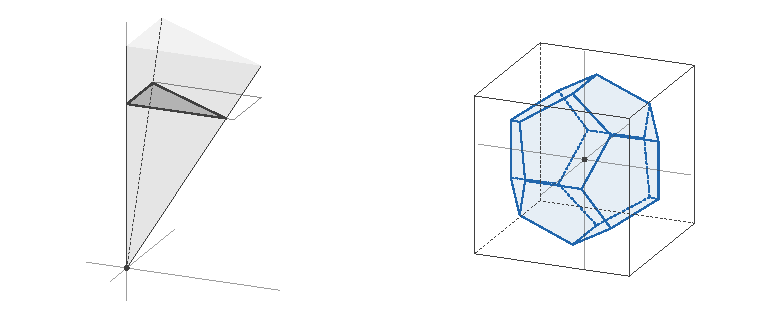
\includegraphics[width=0.82\linewidth]{figures/reduced-ranges}
\caption{The reduced ranges, in the spatial axes of \cref{fig:rid-parametrisation}. Left: the viewing directions kept form a \fc{Grey}{cone (grey)} through the viewing triangle $s,t\ge0$, $\varphi s+\varphi^2t\le1$ in the plane $z=1$ (dark), which lies in the rectangle $[0,2/3]\times[0,2/5]$ of $B_0$ (thin). Right: the box ${[-2/5,2/5]}^3$ of rotation vectors $\mathbf r$ (grey) and the part of it satisfying the twelve rotation comparisons \fc{Plug}{(blue), a dodecahedron}; the fold comparisons, which also involve $s$ and $t$, cut it further.}
\label{fig:reduced-ranges}
\end{figure}

\begin{proposition}[Representative coverage]\label{prop:representative-coverage}
  Every centred geometric configuration has a representative in $D$ with
  the same margin. In particular, a fit exists if and only if one
  exists in $D$.
\end{proposition}
\begin{proof}
  First apply a hole symmetry to the viewing line and the common frame
  to place the representative vector $\mathbf u$ in the cone
  \cref{eq:viewing-cone}. An orientation-reversing
  symmetry is implemented by its negative, with the viewing vector's sign
  reversed, as in \cref{subsec:symmetries-preserve-the-projection-problem}.
  The transformed vector has positive $z$-coordinate, so normalising it gives
  $\mathbf u=(s,t,1)$ satisfying \cref{eq:viewing-triangle} and the first
  two interval bounds of $B_0$.

  Keep $(s,t)$ fixed and choose the maximal-scalar quaternion from
  \cref{eq:rotation-representative-family}. Its positive scalar part
  permits the normalisation $(1,\mathbf r)$, and its comparisons give
  \cref{eq:rotation-comparisons,eq:fold-comparisons} and the remaining
  interval bounds of $B_0$. Every operation preserves the margin, so
  this is the required representative. Conversely, each point of $D$
  specifies an actual viewing line and rotation by the formulas of
  \cref{subsec:parametrisation-of-the-configuration-space}.
\end{proof}

All the inequalities are non-strict. In particular, the argument retains
viewing directions lying in reflection planes, ties between rotation representatives and
equality in the fold comparisons. A configuration can have more than one
representative in $D$; coverage is all that the proof needs.
For a configuration initially allowing displacement, the centering lemma
first preserves the existence of a fit, and the proposition then
puts a centred fit in $D$.

\paragraph{Compactness and the minimum margin.}
The coverage proposition ensures that $D$ is nonempty. Its polynomial
inequalities define a closed subset of the compact rectangle $B_0$,
so $D$ is compact. By \cref{prop:continuity-and-openness}, the margin
therefore attains its minimum on $D$. Representative coverage gives the promised bounded
form of \cref{eq:nieuwland-number-and-margin}:
\begin{equation}\label{eq:nieuwland-number-on-reduced-domain}
  \nu(\mathcal R)=\frac{1}{\displaystyle\min_{c\in D}M_{\mathcal R}(c)}.
\end{equation}
The remaining task is to show that $M_{\mathcal R}(c)\ge1$ throughout $D$.
We will work from the simpler enclosing rectangle $B_0$ and use these
inequalities to set aside regions entirely outside $D$. Their physical
configurations already have representatives in $D$; no classification of these
as fit, touch or poke configurations is needed to set those regions aside.
